\section{Viola Jones Face Detection Algorithm}\label{sec:viola}

Before we proceed into the actual details of the implementation, we discuss the background of viola-Jones Object detection 
framework in this section. Human faces share some similar properties. 
These properties are mapped mathematically to the HAAR features, which are explained in detail below.


The algorithm has four stages as described below:
\begin{itemize}
\item \textbf{Haar feature selection}
The Viola Jones classifier method is based on Haar-like features. The features consist of 
white and black rectangles as shown in Figure~\ref{fig:haar}. These features can be thought of as pixel intensity evaluation sets. 
For each feature, we subtract black region’s pixel value sum from white region’s pixel value sum. 
If this sum is greater than some threshold, it is decided that the region has this feature. 
This is the characteristic value of a feature. We have the Haar features to be used for face detection.

\begin{figure}[h]
  \centering
  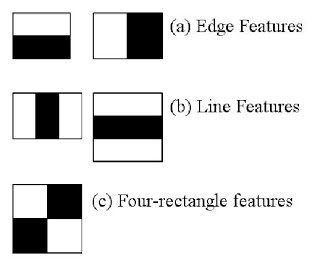
\includegraphics[width=0.5\linewidth]{figs/haar.jpg}
  \caption{Four kinds of HAAR feature rectangles \textnormal{\small }  }
  \label{fig:haar}
\end{figure}

\item \textbf{Integral Image}
The calculation of characteristic value of a feature is an important step in 
face detection. It has to be calculated for every possible pixel region in the given image. 
In order to efficiently determine the value, integral image of the given image is used. 
For any given pixel \emph{(x, y)}, the integral value is the sum of all the pixels above and to 
the left of \emph{(x, y)}, inclusive.
i,e., If \emph{v(x’, y’)} is the value of a pixel at \emph{(x’, y’)},  then the
Integral Sum is given by:

\vspace{0.1in}
\begin{center}
\begin{math}
    IS = \sum\limits_{x'\leqslant  x'y' \leqslant    y'} {v(x’, y’)}
\end{math}
\end{center}



\vspace{0.05in}
Now, the sum of any given region with corner integral pixels A, B, C, D is
\emph{Sum = D + A - B - C} as shown in Figure~\ref{fig:sum}.

\vspace{0.1in}
\begin{figure}[h]
  \centering
  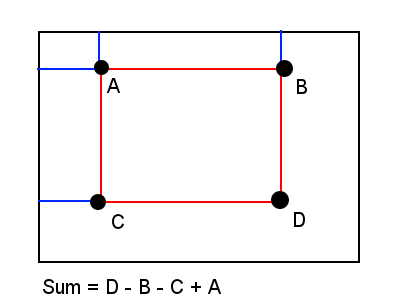
\includegraphics[width=0.5\linewidth]{figs/sum.png}
  \caption{Sum of a sub-window using Integral Image \textnormal{\small }  }
  \label{fig:sum}
\end{figure}

As shown in Figure~\ref{fig:example}, if we want to obtain the sum of 2x3 sub-window, 
integral image involves just 2 additions and 2 subtractions instead of 6 additions.

\begin{figure}[h]
  \centering 
  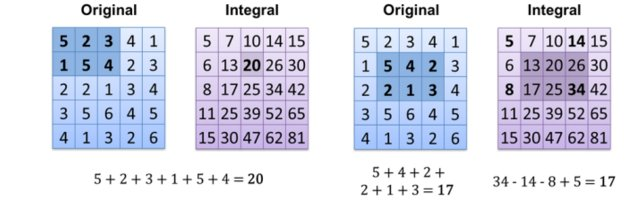
\includegraphics[width=\linewidth]{figs/example.jpg}
  \caption{Example of Integral Image calculation \textnormal{\small }  }
  \label{fig:example}
\end{figure}

\vspace{0.1in}
\item \textbf{Adaboost Algorithm} Adaboost or Adaptive Boosting is a machine learning algorithm 
where the output of weak classifiers is combined into a weighted sum that represents the output 
of a boosted (strong) classifier. This algorithm is used to combine features that cover facial 
characteristics to form a weak classifier. It then creates a string classifier using a group 
of weak classifiers. It further concatenates the strong classifiers to a cascade classifier.


\begin{figure*}[h]
  \centering
  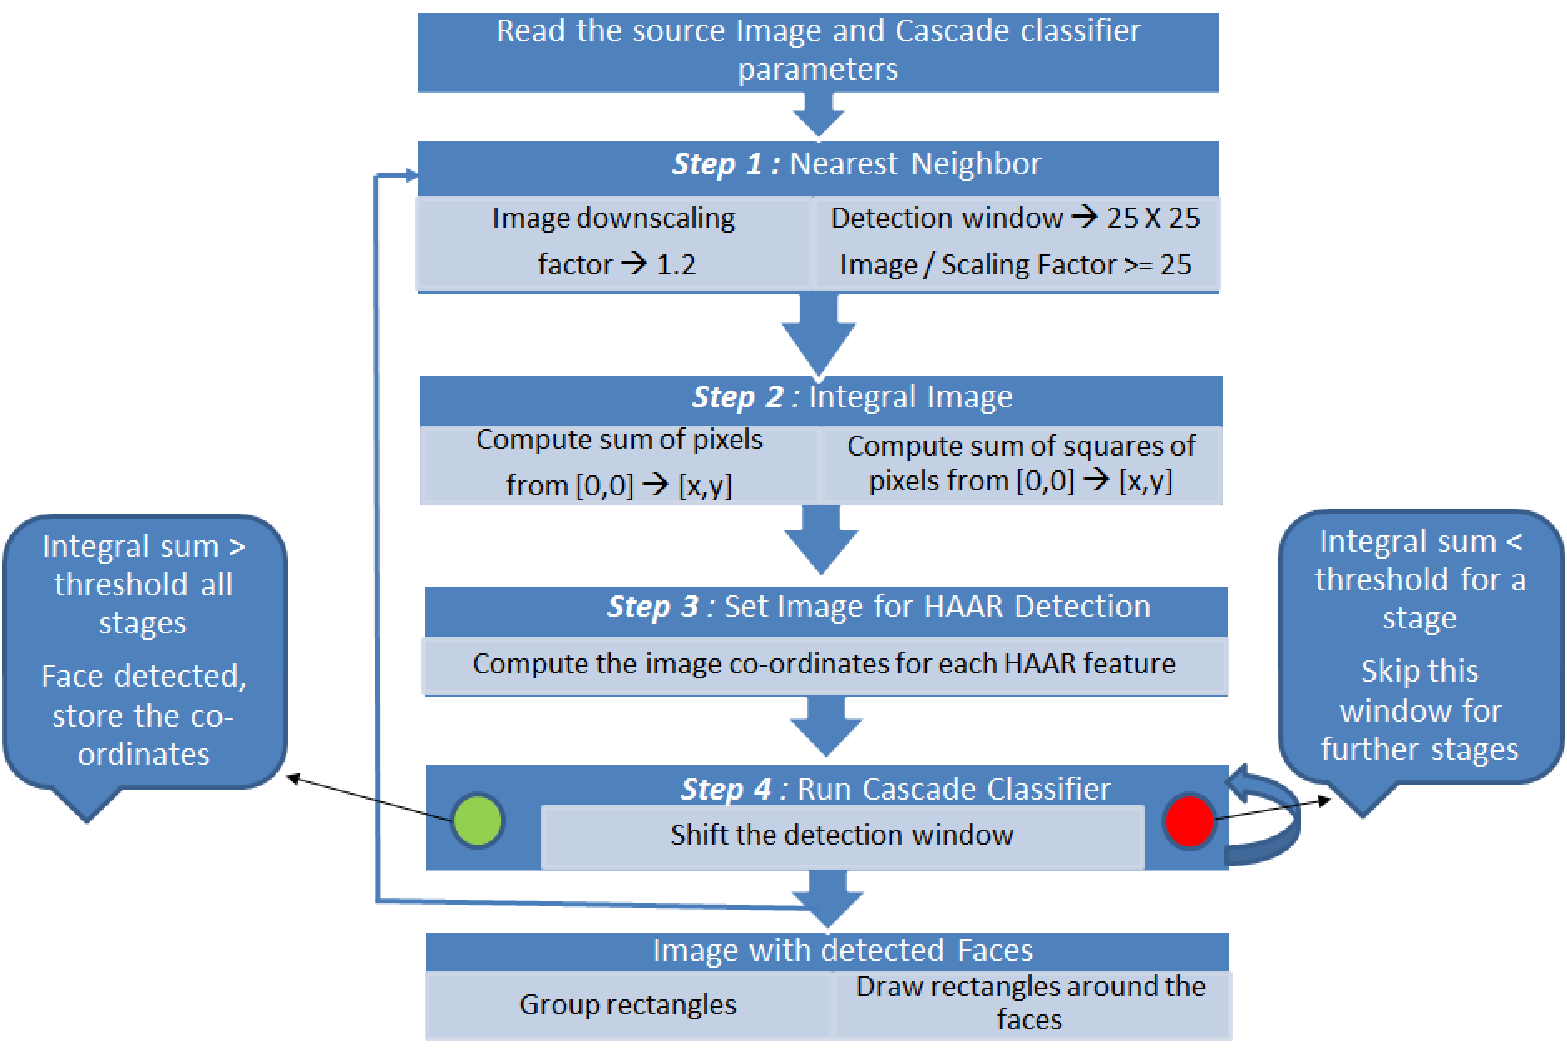
\includegraphics[width=0.75\linewidth]{figs/flow_crop.pdf}
  \caption{Face detection implementation flow }
  \label{fig:flow}
\end{figure*}



\vspace{0.1in}
\item \textbf{Cascade Classifier} A sub-window in the image that passes through the entire cascade 
classifier is detected as human face (Figure~\ref{fig:cascade}). In this project, we used 25 stages in cascade classifier.

\begin{figure}[h]
  \centering
  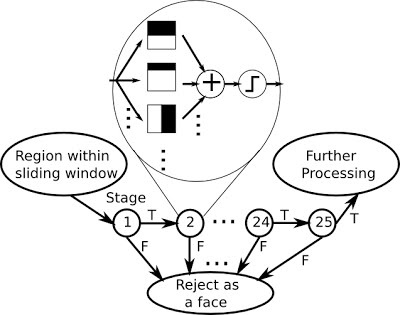
\includegraphics[width=0.8\linewidth]{figs/cascade.jpg}
  \caption{Cascade Classifier \textnormal{\small }  }
  \label{fig:cascade}
\end{figure}

\end{itemize}



